\documentclass[a4paper]{article}

\usepackage[margin=2cm]{geometry}	% For smaller margins
\usepackage[catalan]{babel} 		% Catalan language 
\usepackage{fontspec}				% utf-8 support

\usepackage{float}					% Better positioning 
\usepackage[hidelinks]{hyperref}	% To hide some links
\usepackage{pgfplots}				% Useful to plot data tables
\usepackage{enumitem}				% To use resume in enumerate
\usepackage{multirow}				% Multirow
\usepackage{gensymb} 				% For the degree symbol
\usepackage{graphicx}				% To include images
\usepackage{array}					% To alter column specification
\usepackage{tikz}					% Draw images
\usepackage{pgfplots}				% Add graphs
\usepackage{pgfplotstable}			% To add CSV as tables
\usepackage{amsmath}				% Math symbols
\usepackage{amssymb}

\usetikzlibrary{shapes.misc}

\pgfplotsset{compat=1.13}

\pgfplotstableset{
	create on use/new/.style={
        create col/expr accum={\pgfmathaccuma+1}{0},
        every last row/.style={string type}},
	every head row/.style={after row=\hline},
	display columns/0/.style={column name = Posició },
	display columns/1/.style={column name = T (ºC)},
	display columns/2/.style={column name = $\phi$ (\%)},
	display columns/3/.style={column name = $\vec{v}$ (m/s)},
	use comma,
	dec sep align
}

\newenvironment{questionenum}{%
	\setlist[enumerate]{resume}
	\restartlist{enumerate}
	\newcommand{\question}[1]{
		\begin{enumerate}
			\item\bfseries ##1
		\end{enumerate}
}}{%
}

\setlength{\parindent}{0pt}
\setlength{\parskip}{1em}

\title{
	\textsc{Laboratori de Termodinàmica} \\
	\textsc{Pràctica 5} \\
	Aire humit \\
	\large
	Professor: Jose Luís \\ Grup: 11 }
\author{Joan Marcè Igual \and Esteve Tarragó Sanchís}
\date{13 de novembre de 2016}

\begin{document}
\maketitle

\section{Objectius}

La pràctica té per objectiu la determinació experimental de les propietats d'estat de l'aire humit i l'estudi d'alguns processos de condicionament d'aire com són l'escalfament i el refredament sensible. Es treballarà amb un equip de condicionament d'aire convencional amb compressor inverter i refrigerant R-410A accessible i instrumentat adequadament (dissenyat com equip didàctic). Els estats d'aire humit es determinaran amb un psicròmetre i els processos es visualitzaran en un diagrama psicromètric que també s'utilitzarà per a determinar la resta de paràmetres característics de l'aire: humitat relativa, humitat absoluta, volum específic, entalpia, etc. Finalment es realitzaran els balanços de matèria i energia dels processos estudiats.

\section{Presentació de resultats}

\begin{questionenum}
	\question{Presenteu una taula amb les propietats de l'aire del laboratori. Compareu els diferents sistemes de mesura emprats.}
	
	\begin{table}[H]
		\centering
		\begin{minipage}[t]{0.48\textwidth}
			\centering
			\begin{tabular}{rr}
				$T_{\text{bulb sec}}$ (ºC) & $\phi$ (\%) \\
				\hline
				19,8 & 55,6 
			\end{tabular}
			\caption{Dades obtingudes amb l'\textbf{higròmetre}}
		\end{minipage}
		\hfill
		\begin{minipage}[t]{0.48\textwidth}
			\centering
			\begin{tabular}{rrr}
				$T_{\text{bulb sec}}$ (ºC) & $T_{\text{bulb humit}}$ (ºC) & $\phi$ (\%) \\
				\hline
				22,5 & 26 & 51
			\end{tabular}
			\caption{Dades obtingudes amb el \textbf{psicròmetre}}
		\end{minipage}
	\end{table}
	
	\question{Presenteu dues taules (bateria interior i exterior) que continguin les temperatures, les humitats relatives i les velocitats determinades a diferents punts de la sortida de les bateries i els valors promig calculats.}
	
	\begin{figure}[H]
		\centering
		\begin{tikzpicture}[auto]
			\draw[line width=0.9mm] (-1,1) rectangle (5*1.5 + 1, -2.5);
			\draw[line width=0.9mm] (-1,1.5) rectangle (5*1.5 + 1, -3);
			\draw[rounded corners=15pt] (-1.8,2) rectangle (5*1.5 + 1.8, -3.5);
			\foreach \i in {1,...,20}{
				\draw[thin] (-1, {-3.5*\i/20 + 1}) -- (5*1.5 + 1, {-3.5*\i/20 + 1});
			}
			\foreach \i in {1,...,12}{
				\node[fill=white,circle,draw,minimum size=2.5em] at ({mod(\i - 1, 6)*1.5}, {-1.5*int((\i - 1)/6)}){\i};
			}
		\end{tikzpicture}
		\caption{Esquema de la sortida d'aire a la unitat interior i dels punts de mesura recomanats}
	\end{figure}
	\begin{figure}[H]
		\centering
		\begin{tikzpicture}
			\foreach \i in {0,45,...,360} 
				\draw[black!30] (0,0) -- (\i:4);
			\draw (0,0) circle (4);
			\draw (0,0) circle (1);
			\foreach \i in {1,...,16} {
				\node[fill=white, circle, draw, minimum size=2.5em]
					at ({90-mod(\i - 1, 8)*45}:{3 - int((\i - 1)/8)}){\i};
			}
		\end{tikzpicture}
		\caption{Esquema de la sortida d'airea a la unitat exterior i dels punts de mesura recomanats.}
	\end{figure}
	
	\begin{table}[H]
		\begin{minipage}[t]{0.48\textwidth}
			\centering
			\pgfplotstabletypeset[columns={new,T,H,v}]{data/unitat-interior.csv}
			\caption{Dades de la bateria interior}
		\end{minipage}
		\begin{minipage}[t]{0.48\textwidth}
			\centering
			\pgfplotstabletypeset[columns={new,T,H,v}]{data/unitat-exterior.csv}
			\caption{Dades de la bateria interior}
		\end{minipage}
	\end{table}

    Així doncs per la bateria interior els valors mitjans són els següents:
    \begin{align*}
        & T = 36,3 \degree C \\
        & \phi = 20,3 \% \\
        & \vec{v} = 2,4 m/s
    \end{align*}
    
    Per la bateria exterior els valors mitjans són els següents:
    \begin{align*}
        & T = 16 \degree C \\
        & \phi  = 74,2 \% \\
        & \vec{v} = 2,7 m/s
    \end{align*}

	\question{Representeu al diagrama psicomètric els processos que tenen lloc a les dues bateries i determineu els volums específics, les humitats absolutes i les entalpies a la entrada i a la sortida de les bateries. Presenteu una taula que contingui aquesta informació. Discutiu si s'escau els valors de les humitats absolutes.}
    
    \begin{figure}[H]
        \centering
        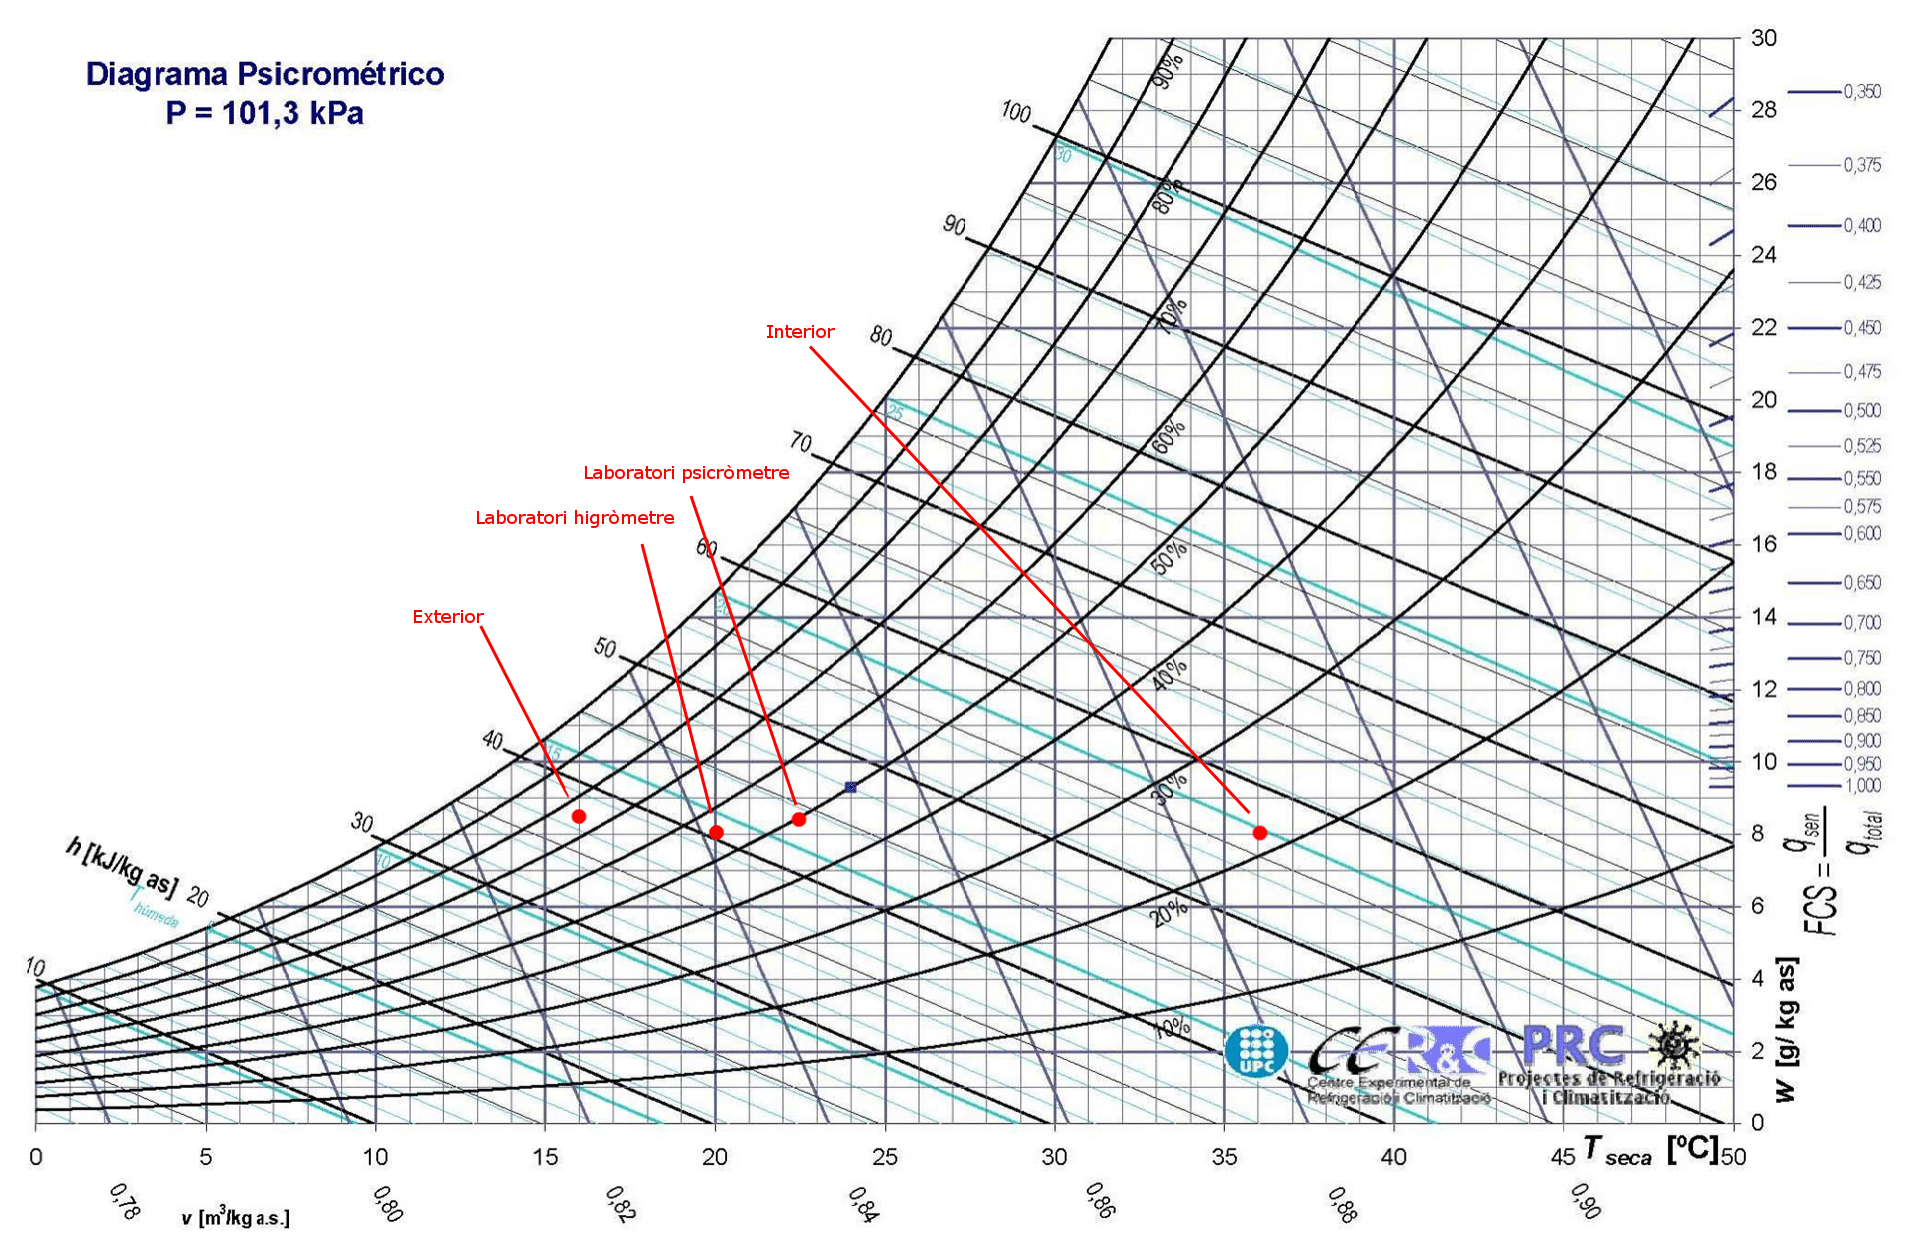
\includegraphics[width=\textwidth]{images/psychrometric}
        \caption{Diagrama psicromètric a pressió atmosfèrica}
    \end{figure}
	
	\question{Determineu el flux màssic d'aire que circula per les dues bateries i les potències frigorífica i calorífica utilitzant les equacions (1) i (2) i les dades extretes del diagrama psicomètric. Discutiu els resultats obtinguts i compareu-los amb les dades facilitades pel fabricant.}
	
	\question{Determineu el cabal volumètric a la sortida de les dues bateries utilitzant l'equació (3) i compareu els resultats obtinguts amb les dades facilitades pel fabricant.}
	
	\question{En cas d'haver determinat dades de l'aire en diferents condicions de funcionament de la màquina, presenteu els resultats de tots els règims de funcionament i discutiu-ne les diferències.}
\end{questionenum}

\end{document}